\scanpage{152}
% position: top
\[
\underbrace{\beta_1=\beta_2}_{\beta}=1-\uuline{\gamma}\chi
\qquad
\alpha=-\beta\unsure{\chi}=-\chi(1-\uuline{\gamma}\chi)
\]
\[
-\chi(1-\uline{\gamma}\chi)\mathrm{id}
+(1-\gamma\chi)(\pi'_1+\pi'_2)+\gamma\pi'_1\otimes\pi'_2
\qquad\gamma\in\mathbb Z
\]
% position: upper calculation
\[
\underbrace{-\chi(1-\gamma\chi)}+2(1-\gamma\chi)\chi+\gamma\chi^2=\chi
\qquad\deleted{2\chi=\chi}\quad\chi=\chi\quad\text{o.K.!}
\]
\[
\deleted{\boxed{\unsure{2=\chi|2\ne\chi}}}
\]
% position: middle right calculation
\[
\begin{aligned}
&-\chi\cdot(1-\gamma\chi)\mathrm{id}_{M_1\otimes M_2}
+(1-\gamma\chi)[\tau_1\otimes\mathrm{id}_2)+\mathrm{id}_1\otimes\tau_2]\\
&\hspace{12em}+\gamma\tau_1\otimes\tau_2\\
&\hspace{12em}\deleted{\unsure{x_1\otimes x_2}}
\end{aligned}
\]
% position: middle lower equations
\[
\left\{\begin{array}{l}
-\chi(1-\gamma\chi)=\chi\\1-\gamma\chi=-1
\end{array}\right.
\qquad
\begin{array}{c}1-\gamma\chi=-1\\\boxed{\gamma\chi=2}\end{array}
\]
\[
\text{\unsure{ou} }2.\qquad\chi=\pm2
\qquad\deleted{\unsure{\chi}}
\]
\[
\unsure{2'}\qquad\chi
\]
% position: lower parameter choice
\[
\chi=2\qquad\gamma=1\quad,\ \beta=-1,\ \alpha=2
\]
donc on \unsure{prend}
\figure{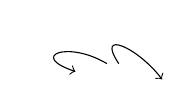
\begin{tikzpicture}
\draw[->] (0,0) .. controls (-.5,.3) and (-1,.1) .. (-.4,-.1);
\draw[->] (.15,0) .. controls (-.15,.45) and (.4,.2) .. (.7,-.2);
\end{tikzpicture}}
% position: lower right operator
\[
\deleted{2\mathrm{id}}\qquad
2\mathrm{id}_{E_1\otimes E_2}
-(\unsure{\pi_{E_1}|\pi'_{E_1}}\otimes\mathrm{id}_{E_2}
+\mathrm{id}_{E_1}\otimes\pi_{E_2})+\pi_{E_1}\otimes\pi_{E_2}
\]
\diagram{\begin{tikzcd}[column sep=large]
x_1\otimes x_2\arrow[r,mapsto]&
\begin{gathered}
2x_1\otimes x_2\unsure{-|+}\pi_1(x_1)\otimes x_2-x_1\otimes\pi_2(\unsure{x_2|x_1})\\
{}+\pi_1(x_1)\otimes\pi_2(x_2)
\end{gathered}
\end{tikzcd}}
% position: bottom left
\[
\overline{x}_1=T_1\psi_1(x_1)-x_1=x_1-\pi_1(x_1)
\]
\[
\pi_1(x_1)=2x_1-T_1\psi_1(x_1)
\]
% position: bottom right cancelled expression
\[
\deleted{\equiv x_1\otimes x_2+(\overline{x}_1\otimes\overline{x}_2)}
\]
\margin{151}
